\chapter{Implementation}

\section{PRA Solver Integration and Abstraction}
The first major challenge in developing a web-based ecosystem for PRA tools is tool integration. Integrating PRA tools is challenging because the supported tools differ in implementation language, invocation style, and input/output format. Some tools are closed source and available only as standalone executables, while others are open-source and can be customized as needed. To hide this complexity, the platform uses an adapter layer and a uniform asynchronous job based API. All requests are first validated against semantic schemas to reject malformed models and reduce the risk of script injection. After a request is accepted, the API immediately returns a job ID that can later be used to check job status or retrieve results. For decomposed event tree runs, the system may also return multiple job IDs associated with the event sequences.

For tools distributed as executables, both open-source and closed source solver binaries, together with their runtime dependencies, are packaged into the same container image as the worker service. This gives each worker direct local access to the solver. Users submit the model in the tool's native format, most commonly OpenPSA XML, but also tool specific formats such as JSInp for SAPHSOLVE, S2ML+SBE for XFTA, or .fta for FTREX, along with optional tool specific settings. If no settings are provided, default values are applied automatically. Because the worker services are written in TypeScript and accept JSON request bodies, raw model files are transmitted as base64 encoded strings. Base64 encoding allows file contents to be sent safely as printable text inside JSON. After receiving a request, the worker decodes the base64 data, writes it to a temporary file with a random name and the correct extension, constructs the same command line flags that the solver expects in normal CLI use, and invokes the executable through Node.js's child\_process.exec() method. The solver output is captured in a temporary result file, the contents of which are then to the object storage, and the temporary input and output files are then deleted.

For direct JSON based quantification, the platform currently supports SCRAM and PRAXIS \cite{praxis} without launching an external solver executable. SCRAM is written in C++, while PRAXIS is written in Rust and supports both CPU and GPU based Monte Carlo probability estimation. PRAXIS has been reproduced from a prior research work on data parallel Monte Carlo probability estimation \cite{arjun_2026}, because the original AGPL licensed implementation \cite{arjun_mcscram} could not be directly integrated into the MIT licensed distributed system as a solver. For both SCRAM and PRAXIS, native Node addons are written around the I/O, settings, and quantification classes/structs needed by the workers. A Node addon is ordinary C++ or Rust code compiled against the Node.js Addon API (Node API/N-API) \cite{napi}. Instead of producing an executable, the normal build system (e.g., CMake for C++ or Cargo for Rust) produces a \texttt{.node} shared library. This library can be imported directly into the TypeScript worker services. The addon exposes wrapper functions that map JSON fields to native C++ or Rust objects, call the underlying quantification routines, and map the native result objects back to JSON. In this way, the system keeps native code performance while still exposing a uniform TypeScript interface.

When users select SCRAM or PRAXIS, they submit the model in the OpenPRA JSON Model Exchange Format (MEF) \cite{openpra_documentation}, which was developed from the non-LWR technical elements standard ASME/ANS RA-S-1.4-2021 \cite{non_lwr_standard}. The model contains four main objects: \textbf{DA} - data analysis information, such as failure mode names, probabilities/frequencies, and distributions; \textbf{SA} - systems analysis information, including fault tree logic, \textbf{IE} - initiating event information, such as event names, grouping, and frequencies; and \textbf{ESA} - event sequence analysis information, including event tree logic, functional events, linked top events, failure/success/bypass states, and sequence names. Users also provide quantification settings, such as algorithm choice, requested analysis types, approximations, truncation limits, hardware selection etc. The request is routed to the appropriate worker function, which loads the required \texttt{.node} library, maps the JSON input to native data structures, executes the quantification, converts the native result structure back to JSON, and stores the result.

To execute native quantification reliably, the workers use a multi process design. Running a long native computation on the main Node.js thread would block the event loop and prevent the RabbitMQ connection from sending heartbeats. After a timeout, RabbitMQ may treat the worker as disconnected, drop the connection, and requeue the job. One possible solution is to offload the work to a separate thread, but that would require two threads per worker and leave the main thread largely idle. Instead, the parent process keeps the RabbitMQ connection alive, while a child process loads the addon and performs the quantification in its own memory space. This avoids dropped connections without wasting worker threads. Figure~\ref{fig:solver-integration} shows the internal architecture and workflow of each worker/consumer service.

\begin{figure}[]
  \centering
  \includesvg[width=1.10\textwidth]{5-implementation/plots/solver-integration.svg}
  \caption{Internal architecture and workflow of the worker/consumer services for PRA solver integration and result handling.}
  \label{fig:solver-integration}
\end{figure}

Event tree decomposition is supported in three ways, depending on the capabilities of the selected tool:
\begin{itemize}
    \item \textbf{Fault tree only tools (e.g., FTREX and XFTA):} The event tree is transformed into the logical OR of its individual event sequences. Each sequence is then converted into a fault tree and quantified independently. The final event tree result is obtained by OR-combining the sequence results.
    \item \textbf{Closed source tools with event tree support:} The original event tree input file is split into separate inputs, one per event sequence. Each sequence is quantified as an independent job, and the partial results are stitched back together afterward.
    \item \textbf{Open source tools with internal model access:} A lightweight addon first generates only the tool's internal PDAG representation for the full event tree. That PDAG is then partitioned by event sequence and the chunks are distributed to different workers. This avoids regenerating the PDAG for every sequence and reduces repeated preprocessing cost.
\end{itemize}

Result aggregation is also automated. Workers processing decomposed jobs use distributed coordination to determine when all related sequence jobs have finished. The final worker or coordinator then performs deterministic aggregation by extracting the required fields from the individual results according to predefined output schemas and stitching them into the final response. As a result, even when the system internally creates many sub-jobs, the user facing workflow remains simple: submit once, track the returned job ID(s), and retrieve the final result later.

\section{System Architecture Implementation}
\label{sec:sys-arch-implementation}
The deployed system combines three architectural styles: (i) a 4 tier client-server flow for non-quantification requests, (ii) a microservice based deployment where each component is packaged and scaled independently, and (iii) an event driven pipeline for long running quantification and tool execution jobs. From left to right, in Figure~\ref{fig:system-implementation}, the main components are the client, the reverse proxy, the API gateway (server backend), the message broker, the worker services, and the storage layer.

A client can be a web frontend, a lightweight library, or any code that can send HTTP(S) requests to the exposed API endpoints. Incoming requests first pass through a containerized reverse proxy:
\begin{itemize}
    \item \textbf{Traefik (multi node deployments):} used because it integrates well with on-premise cluster based deployments by providing dynamic routing and service discovery, built-in load balancing, and automated TLS certificate management.
    \item \textbf{Nginx (single node deployments):} used as the primary load balancer and reverse proxy. When all services run on a single machine, a static upstream configuration is sufficient for distributing requests across API gateway replicas.
\end{itemize}

\begin{figure}[]
  \centering
  \includesvg[width=\textwidth]{5-implementation/plots/system-implementation.svg}
  \caption{System implementation architecture showing the deployed components and their associated technology stack.}
  \label{fig:system-implementation}
\end{figure}

The reverse proxy intercepts client requests, applies routing, TLS, load-balancing as needed, and forwards traffic to an instance of the API gateway. The API gateway is implemented in NestJS \cite{noauthor_documentation_nodate}, a Node.js \cite{Node} based framework and written in TypeScript \cite{starting}.
The gateway is not only an HTTP entry point but also the place where request routing and the core backend logic live:
\begin{itemize}
    \item \textbf{Routing logic:} inspects the request URL and request type (non-quantification vs. quantification or execution), and for quantification/execution requests also identifies which tool or workflow is requested.
    \item \textbf{Business logic:} handles control plane operations such as creating and updating job records, storing and returning job status and error information, and returning metadata required to locate inputs or outputs.
    \item \textbf{Producer:} for long running compute requests, the gateway forwards the request to an internal producer module (also implemented inside NestJS). The producer serializes the request body into a message buffer and publishes it to the message broker.
\end{itemize}
Table~\ref{tab:endpoints} lists the main API entry points, together with their HTTP methods and a short description. The API gateway, business logic, and producer logic are deployed together as a single containerized backend service. Communication follows two complementary patterns:
\begin{itemize}
    \item \textbf{Synchronous HTTP APIs:} Used for non-quantification operations and job control, for example: submit a job and receive an acknowledgement, query job status, and retrieve stored results once available).
    \item \textbf{Asynchronous messaging (event driven):} Used for quantification and execution jobs that may take substantial time. These jobs are queued and processed by workers in the background.
\end{itemize}

\begin{landscape}
\begin{longtable}{@{}lll@{}}
\caption{Main entrypoints exposed by the API gateway.}
\label{tab:endpoints}\\
\toprule
\textbf{Endpoint} & \textbf{Methods} & \textbf{Description} \\
\midrule
\endfirsthead
\caption*{Table \thetable{} (continued).}\\
\toprule
\textbf{Endpoint} & \textbf{Methods} & \textbf{Description} \\
\midrule
\endhead
\bottomrule
\endfoot
%
\multicolumn{3}{@{}l}{\textbf{Executable Solver Submission}}\\
\midrule
\texttt{/q/execute/scram} & POST & Submit an executable based SCRAM quantification job \\
\texttt{/q/execute/ftrex} & POST & Submit an FTREX executable quantification job \\
\texttt{/q/execute/xfta} & POST & Submit an XFTA executable quantification job \\
\texttt{/q/execute/saphsolve} & POST & Submit a SAPHSOLVE executable quantification job \\
\texttt{/q/execute/<tool>?distributedSequences=true} & POST & Submit an executable task using event tree decomposition \\
\addlinespace
\multicolumn{3}{@{}l}{\textbf{Direct JSON Quantification}}\\
\midrule
\texttt{/q/quantify/scram} & POST & Submit a direct JSON based SCRAM quantification job \\
\texttt{/q/quantify/praxis} & POST & Submit a direct JSON based PRAXIS quantification job \\
\texttt{/q/quantify/<tool>?distributedSequences=true} & POST & Submit a quantification job using event tree decomposition \\
\addlinespace
\multicolumn{3}{@{}l}{\textbf{Job Retrieval and Monitoring}}\\
\midrule
\texttt{/execute/results/\{job\_id\}} & GET & Retrieve results for an executable based job \\
\texttt{/quantify/results/\{job\_id\}} & GET & Retrieve results for a direct quantification job \\
\texttt{/execute/status/\{job\_id\}} & GET & Retrieve status for an executable based job \\
\texttt{/quantify/status/\{job\_id\}} & GET & Retrieve status for a direct quantification job \\
\texttt{/execute/input/\{job\_id\}} & GET & Retrieve the submitted input for an executable based job \\
\texttt{/quantify/input/\{job\_id\}} & GET & Retrieve the submitted input for a direct quantification job \\
\end{longtable}
\end{landscape}

Asynchronous processing is implemented using RabbitMQ \cite{RabbitMQ}, an AMQP based message broker \cite{enwiki:1297038479}. RabbitMQ was selected because it provides reliable delivery with acknowledgements, flexible routing via exchanges  keys, durable queues, and operational features such as dead lettering and queue policies.

The producer publishes each job to one of two main queue classes: (i) quantification queue(s) and (ii) executable queue(s). In practice, each class may contain multiple (possibly temporary) queues, and RabbitMQ routes messages to the correct queue using the exchange routing key, i.e., the key indicates which queue family a message belongs to.

Queues are configured to be durable and messages are published as persistent. This ensures that both the queue definitions and the messages survive broker restarts and crashes, because RabbitMQ writes the relevant data to disk instead of memory. In addition, queue policies such as maximum queue length and message TTL are used. If a queue overflows or a message stays unprocessed for too long, it is moved to a dead letter queue instead of being endlessly re-queued, which would otherwise allow a stuck job to starve other jobs. RabbitMQ itself is deployed as a containerized service.

Compute is performed by separate worker services. Each worker service is a containerized NestJS application that runs RabbitMQ consumers. These worker services are kept separate from the API gateway. When a consumer is free and a message is available, it: (i) consumes the message, (ii) parses its contents to identify the job type and (iii) invokes the corresponding worker function.

Two execution paths, i.e., two types of worker functions are supported:
\begin{itemize}
    \item \textbf{Quantification jobs:} The worker passes the received JSON payload to a Node.js wrapper (Node addon). The addon maps the JSON data into native representations (C++ classes or Rust structs), executes the PRA quantification in the native codebase, and then converts the resulting objects back into JSON for storage.
    
    \item \textbf{Executable jobs:} The request payload contains the model encoded in Base64 format. The worker decodes it, converts it into the solver specific input format (e.g., OpenPSA for most solvers and JSInp for SAPHSOLVE), writes the model to corresponding temporary input file(s), and invokes the solver via a child process with the required command line flags and the directory of the temporary input file(s). The solver generates output files, which are read back by the worker and prepared for storage.
\end{itemize}

Workers are containerized together with the required solver executables and their dependencies. They are deployed as separate services so they can be scaled independently. For example, quantification workers can be scaled separately from executable workers.

Two non relational storage systems are used to match different access patterns:
\begin{itemize}
    \item \textbf{MongoDB \cite{MongoDB}:} Stores structured metadata such as job identifiers, submission parameters, timestamps, and run status/progress information.
    \item \textbf{MinIO \cite{minio}:} Stores large artifacts such as uploaded input files and generated output reports. MinIO provides a web interface that can be used to browse and download stored objects.
\end{itemize}
Both MongoDB and MinIO are deployed as containerized services and can be scaled separately from the compute layer. All major components: reverse proxy, API gateway, RabbitMQ, worker services, and storage services are packaged as Docker containers \cite{docker}. The system supports two deployment modes:

\begin{itemize}
    \item \textbf{Single node deployment:} all containers run on a single machine using standard Docker networking. In this mode, Nginx is used as the reverse proxy because the setup is static and no cross node service discovery is required.

    \item \textbf{On-premise multi node deployment using Docker Stack / Swarm:} the system is deployed as a Docker Stack, allowing services (API gateway replicas, worker replicas, RabbitMQ, and storage services) to be scheduled across multiple nodes. In this mode, overlay networks are used so that containers running on different machines can communicate as if they were on the same logical network. Overlay networking also enables clean network segmentation (e.g., restricting internal service-to-service traffic to the overlay network while exposing only the reverse proxy externally). Traefik is used in this mode because it can automatically discover services and apply routing and load-balancing rules dynamically as services scale up or down.
\end{itemize}

Overall, this containerized and modular design keeps services loosely coupled and independently scalable: the reverse proxy, backend, broker, worker pools, and storage can be scaled or updated without requiring the whole system to be redeployed.

\section{Scalability and Resource Management Implementation}
The system uses a manually deployed container based architecture defined through YAML files. Deployment begins by creating a Docker network. A single reverse proxy is then deployed to listen for incoming requests on ports 43 and 8080. After that, the core services are started in sequence: one RabbitMQ instance for job brokering, followed by MongoDB and MinIO. RabbitMQ currently runs as a single instance, whereas MongoDB and MinIO are deployed with multiple instances across multiple nodes. The worker tier is deployed next. At present, the system runs 128 workers, and each worker has direct access to the required solvers. Finally, multiple producer instances are deployed, and the reverse proxy load balances requests across them to maintain high throughput.

On the compute side, scalability is achieved by running many producers and workers in parallel rather than through fully automatic orchestration. Resource management focuses on assigning jobs to suitable hardware and preventing individual analyses from exhausting shared capacity. Workers can be deployed on specialized nodes, such as high memory nodes for ZBDD operations and standard CPU nodes for routine quantification. Resource limits are used to prevent memory intensive jobs from overwhelming a node. At present, GPU enabled executions are available only for single node based deployments and are not yet supported in on-premise cluster deployments.

Job scheduling also includes a priority and fair share mechanism. Each job can be assigned a priority level from 1 to 5, and each user is limited to a total of 50 priority points within a one hour window. This prevents any single user from monopolizing the system while still allowing urgent jobs to be submitted with higher priority.

Storage scalability is provided by MinIO in distributed mode and by MongoDB sharded clusters with hashed sharding keys, which distribute metadata evenly across replica sets. Together, these components allow the platform to support concurrent submissions, distribute quantification workloads across many workers, and store large result sets efficiently.

\section{Security and Access Control Implementation}
Security is implemented through JWT based authentication and role based access control. The API Gateway validates JWT tokens for every request, extracting user roles and permissions that determine access to specific solvers, models, and analytical services. Access to jobs and results is controlled through the same authentication and role based authorization, and ownership checks, which prevent unauthorized cross access to stored data.

All PRA models and results are encrypted using AES 256 encryption by default in MinIO object storage. The system encrypts sensitive nuclear facility data before storage and applies Brotli \cite{brotli} compression to reduce bandwidth.

Audit logging captures every significant action: model submissions, job executions, and result accesses with immutable timestamps and user identifiers. Logs are stored in a secure format for compliance and monitoring. Session management enforces automatic timeout after 30 minutes of inactivity, requiring re-authentication for continued access.

\section{Operational Monitoring, Testing, and Documentation}
The testing suite consists of Jest for unit tests and Supertest for API integration testing. Unit tests cover individual adapter functions and schema validators, while end-to-end tests verify full quantification pipelines, from job submission through result retrieval, using reference PRA models with known expected results.

Monitoring is implemented through Prometheus metrics that track number of queued jobs, worker utilization, error rates, and job completion times. Grafana dashboards provide real-time visibility into system health. Alert rules trigger notifications when critical thresholds are exceeded, such as increased queue backlogs or job failure rates.

Maintenance includes automated cleanup of temporary storage files. Health checks validate service availability every 30 seconds, with failed containers automatically restarted by Docker. Troubleshooting documentation provides step-by-step guidance for common failure scenarios, including solver specific error codes and recovery procedures.

All system components include comprehensive logging using structured JSON format, with unique IDs tracing requests across service boundaries. Log aggregation through the ELK stack enables efficient debugging and operational analysis.

Documentation forms an integral part of the implementation, with comprehensive guides covering system architecture, API references, deployment procedures, and operational practices. 

%Fig. \ref{fig:swagger_doc} shows the interactive API documentation generated by Swagger for the distributed system microservice, detailing its available endpoints, supported request methods, and operational descriptions.
%\begin{landscape}
\begin{figure}
    \centering
    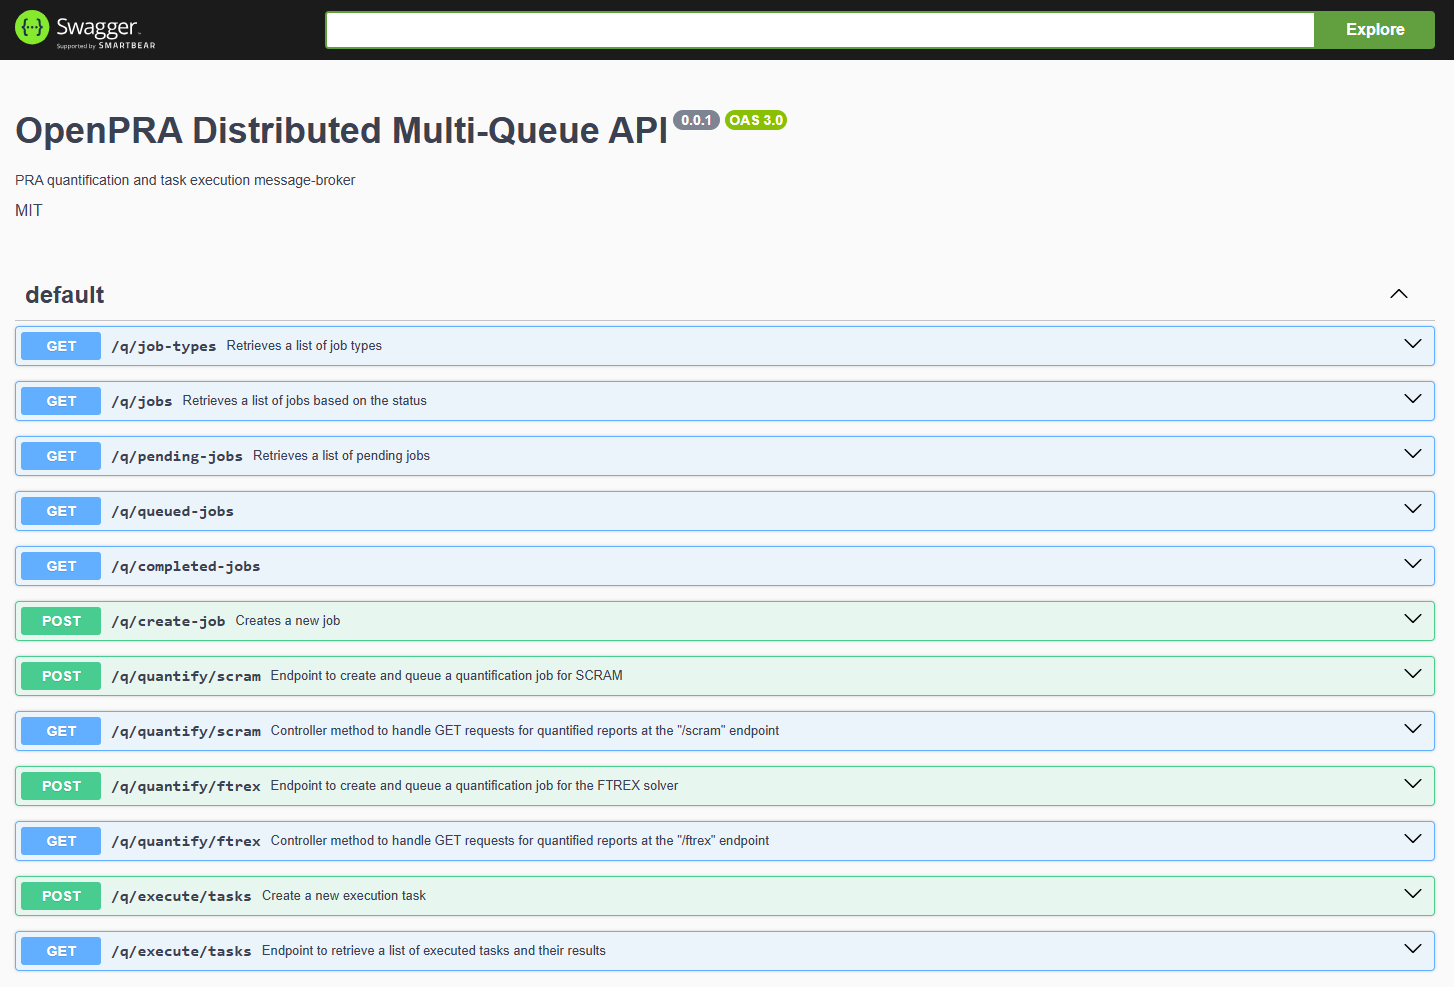
\includegraphics[width=1.3\textwidth]{5-implementation/plots/swagger_doc.png}
    \caption{Interactive API documentation detailing the endpoints available in the distributed networked system.}
    \label{fig:swagger_doc}
\end{figure}
\end{landscape}